\documentclass[10pt]{article}

%---------------------------------------------------------------------
\usepackage[a4paper, headsep=-4in,bindingoffset=0in,%
left=2.5cm,right=2.5cm,top=2.5cm,bottom=2.5cm,%
footskip=.25in]{geometry}
\newcommand{\textBF}[1]{%
    \pdfliteral direct {2 Tr 0.3 w} %the second factor is the boldness
     #1%
    \pdfliteral direct {0 Tr 0 w}%
}
\usepackage{multirow}
\usepackage{soul}

\usepackage{xr}
\externaldocument{main}
\def\Plus{\texttt{+}}
%\usepackage[english]{babel}   
\usepackage[utf8]{inputenc}  
\usepackage[font=scriptsize]{caption}
\usepackage{tabularx}
%\DeclareCaptionFont{6pt}{\fontsize{6pt}{6pt}\selectfont}
\captionsetup[figure]{font={stretch=1}}  
%\usepackage{sectsty}
\usepackage{subcaption}
\usepackage{wrapfig}
\usepackage{layout}
\usepackage{graphicx}
\usepackage{verbatim}
\usepackage{listings}
\usepackage{mathptmx}

\usepackage{booktabs}
\usepackage{etoolbox}


\usepackage{lmodern}
\usepackage[T1]{fontenc}
\usepackage[backend=biber,style=apa,sorting=none]{biblatex}
\addbibresource{paperpile.bib}
%\pagenumbering{gobble}
\pagenumbering{arabic}

\graphicspath{{figs/}}
\setlength{\topmargin}{-10pt}
%\renewcommand{\baselinestretch}{1.5}

\usepackage{indentfirst}
\setlength{\parindent}{1cm}
\usepackage[table]{xcolor}

\setlength{\headsep}{1pt}
%---------------------------------------------------------------------

\begin{document} 



\section*{Supplementary Results}

\begin{figure}[ht]
\centering
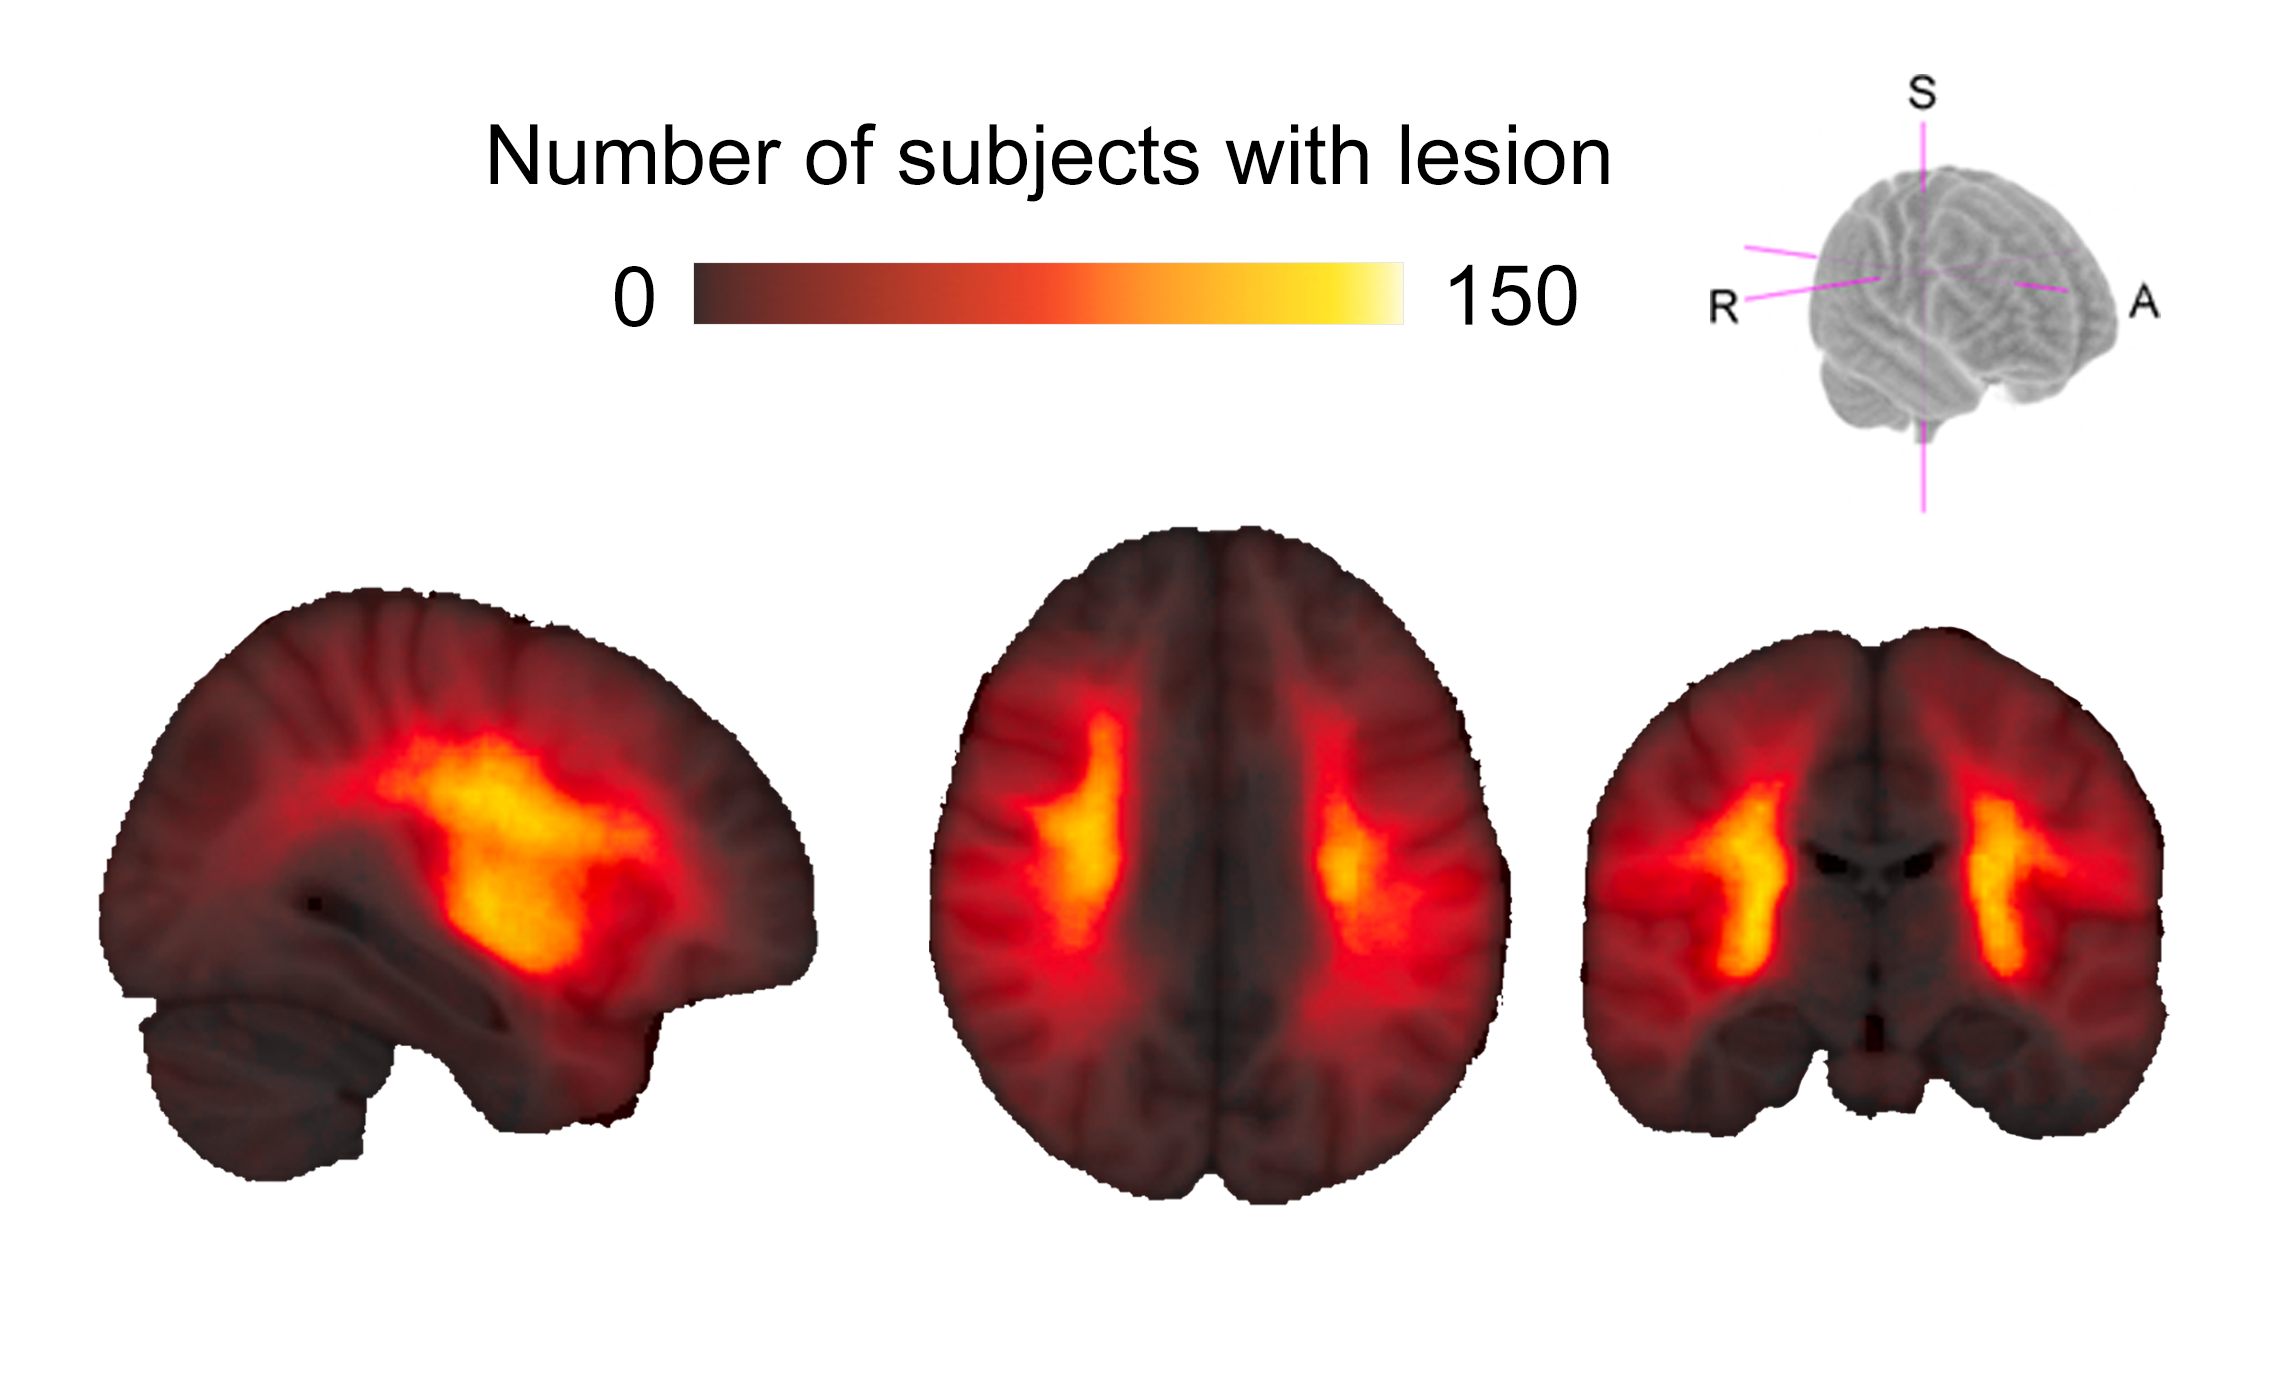
\includegraphics[width=0.8\linewidth]{figures/distribution_lesions.png}
\caption{Distribution of lesions in ENIGMA cohort.}
\label{lesiondist}
\end{figure}

\begin{figure}
\begin{subfigure}{0.5\textwidth}
  \centering
  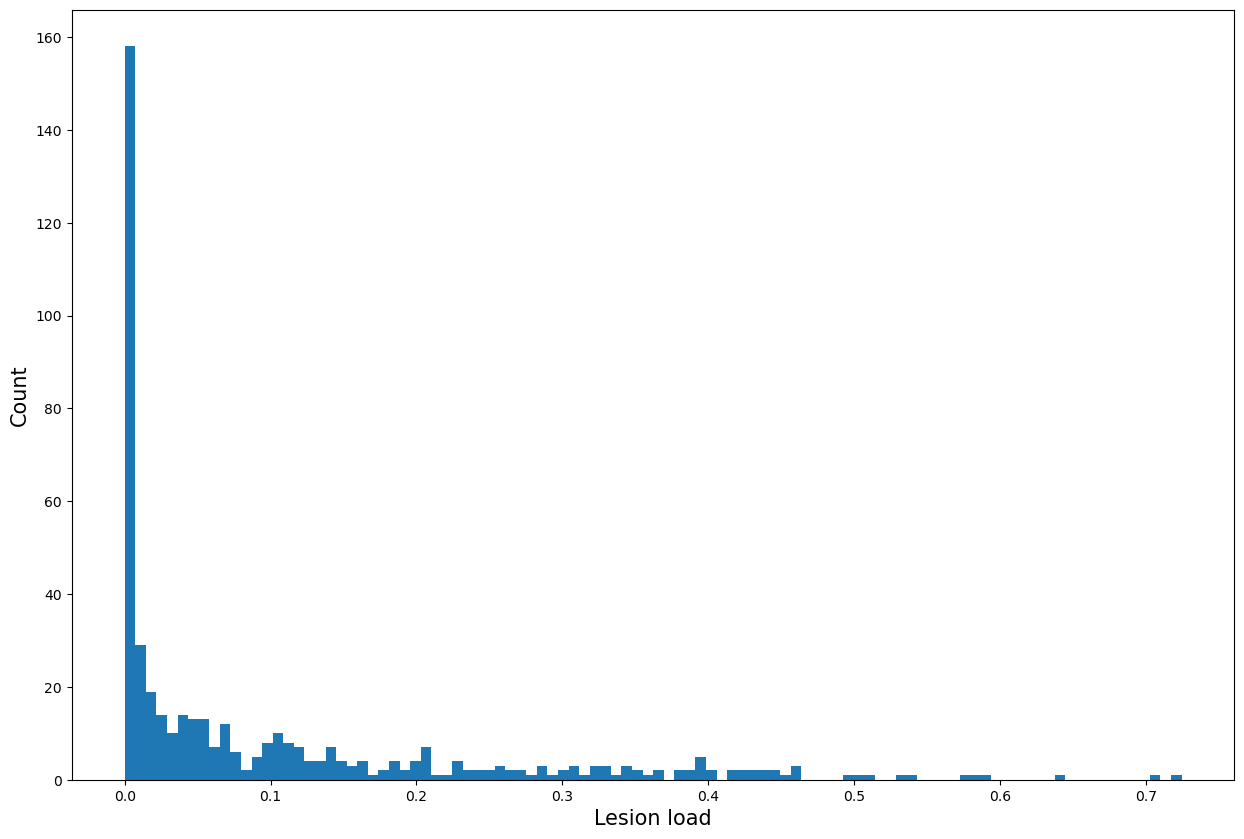
\includegraphics[width=1\linewidth]{figures/m1_lesionload.png}
  \caption{M1-CST lesion load distribution.}
  \label{fig:sfig1}
\end{subfigure}
\begin{subfigure}{0.5\textwidth}
  \centering
  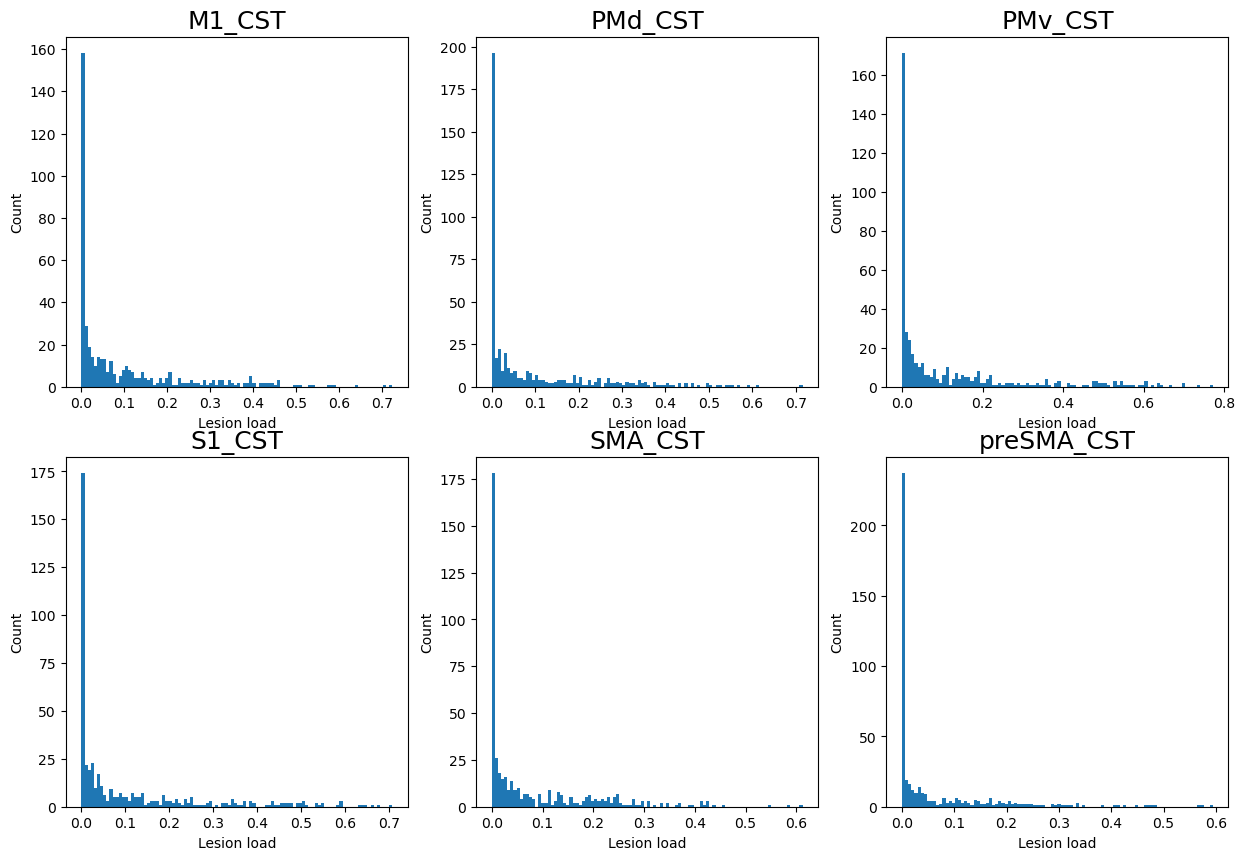
\includegraphics[width=1\linewidth]{figures/all_lesionload.png}
  \caption{Ipsilesional sensorimotor tract template (SMATT) lesion load distribution.}
  \label{fig:sfig2}
\end{subfigure}
\begin{subfigure}{1\textwidth}
  \centering
  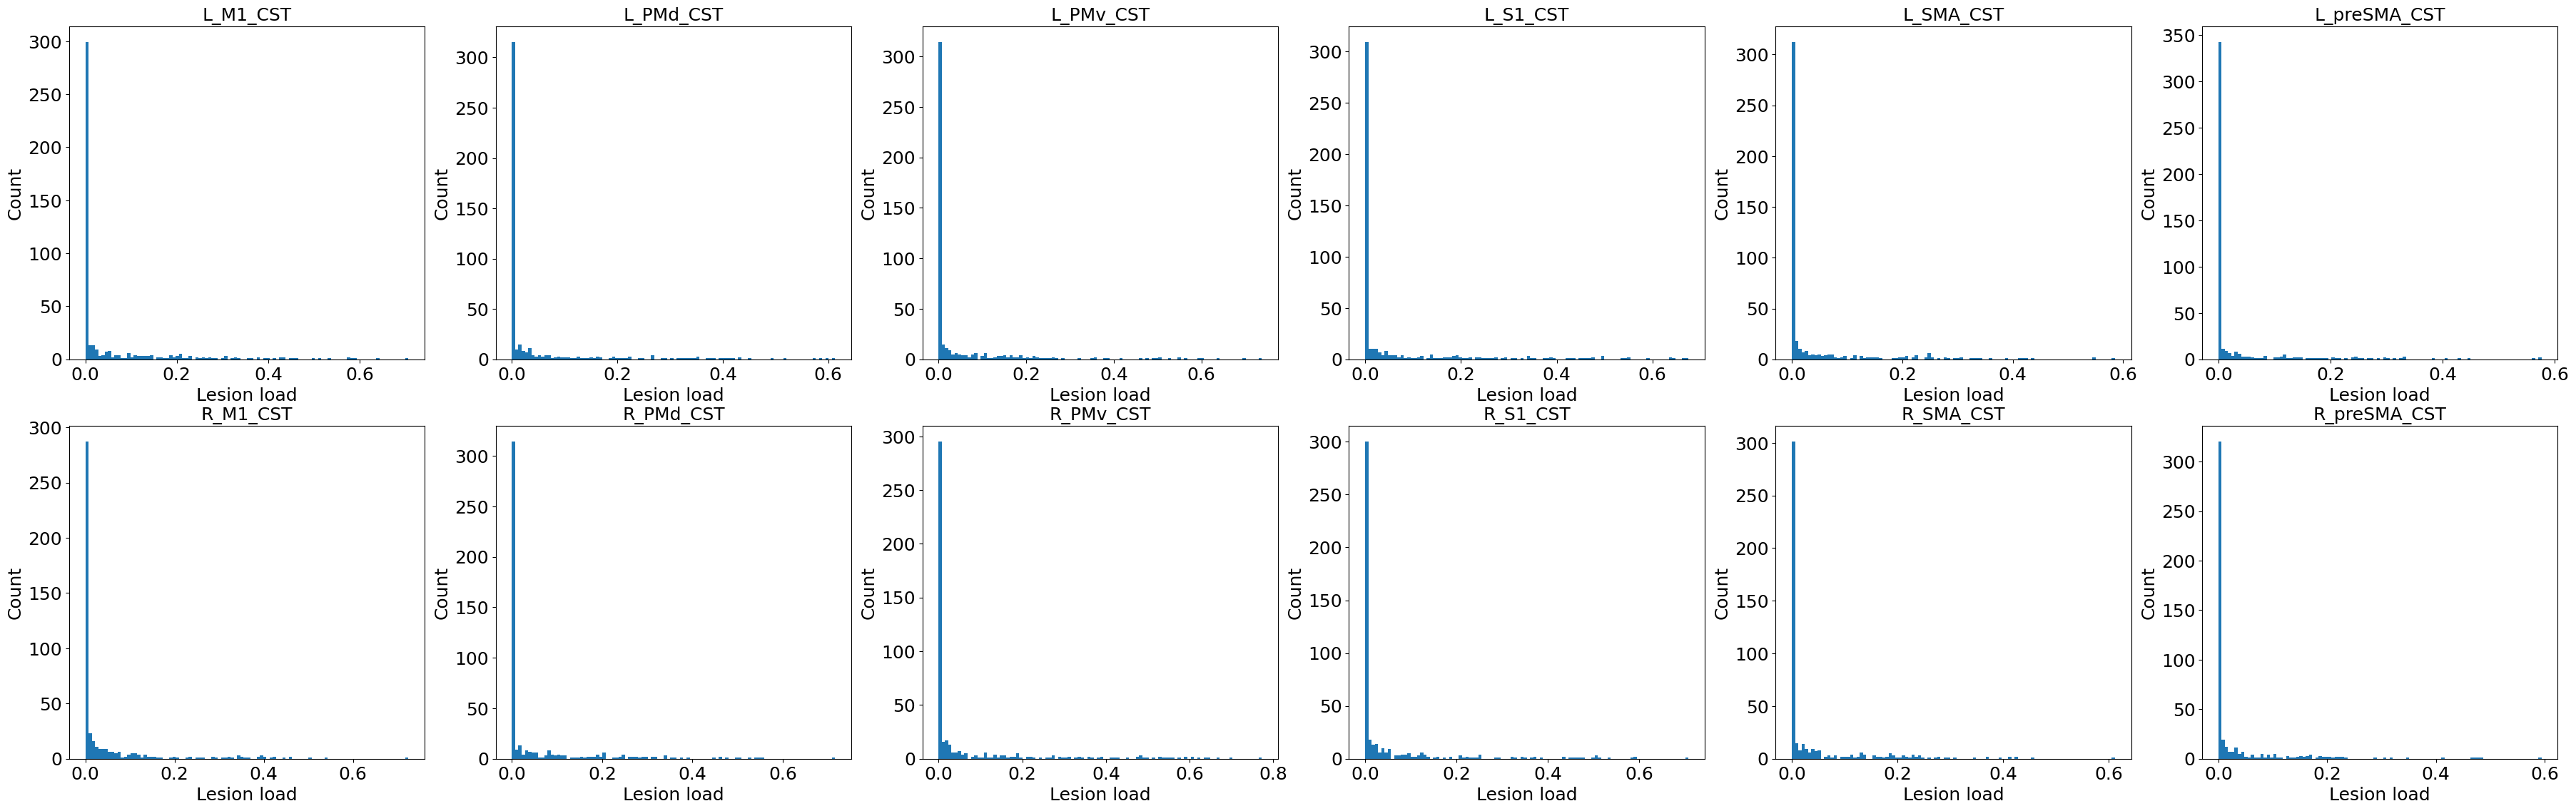
\includegraphics[width=1\linewidth]{figures/all2h_lesionload.png}
  \caption{Left and right hemisphere sensorimotor tract template (SMATT) lesion load distribution.}
  \label{fig:sfig2}
\end{subfigure}
\caption{Distribution of lesion load variables for chronic subjects.}
\label{lesion_load_dist}
\end{figure}


\begin{figure}[ht]
\centering
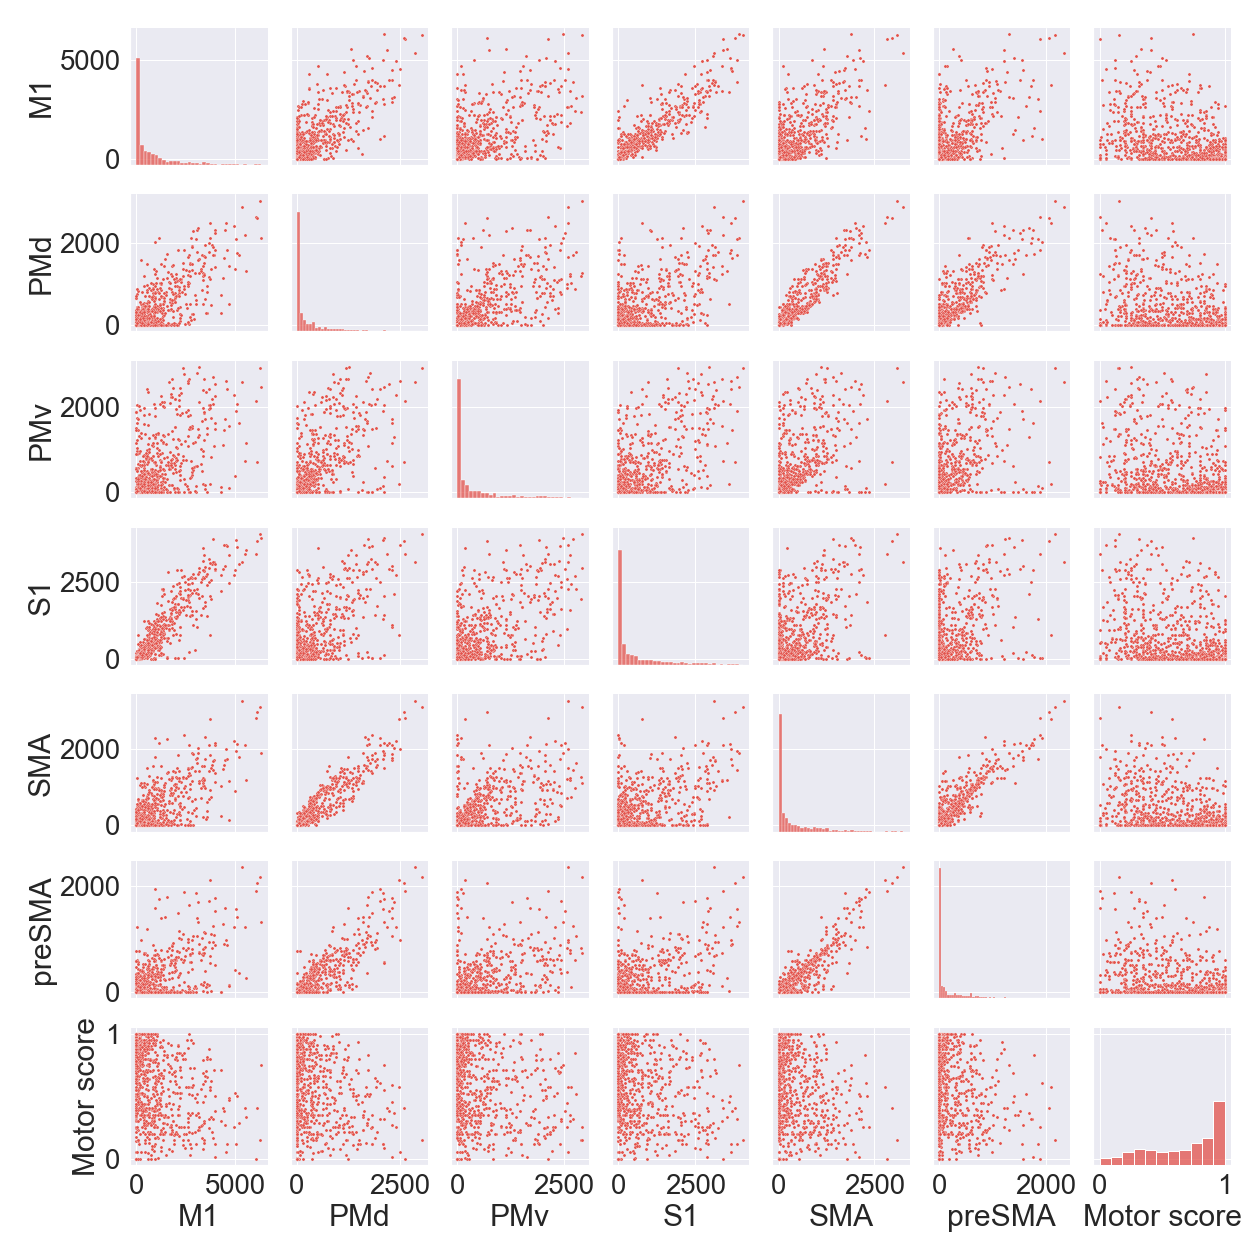
\includegraphics[width=0.8\linewidth]{figures/SMATT_scatterplts.png}
\caption{Correlations between lesion load calculated for each ipsilesional tract in the sensorimotor area tract template atlas.}
\label{smatt_pairwise_correlations}
\end{figure}

\begin{figure}[ht]
\centering
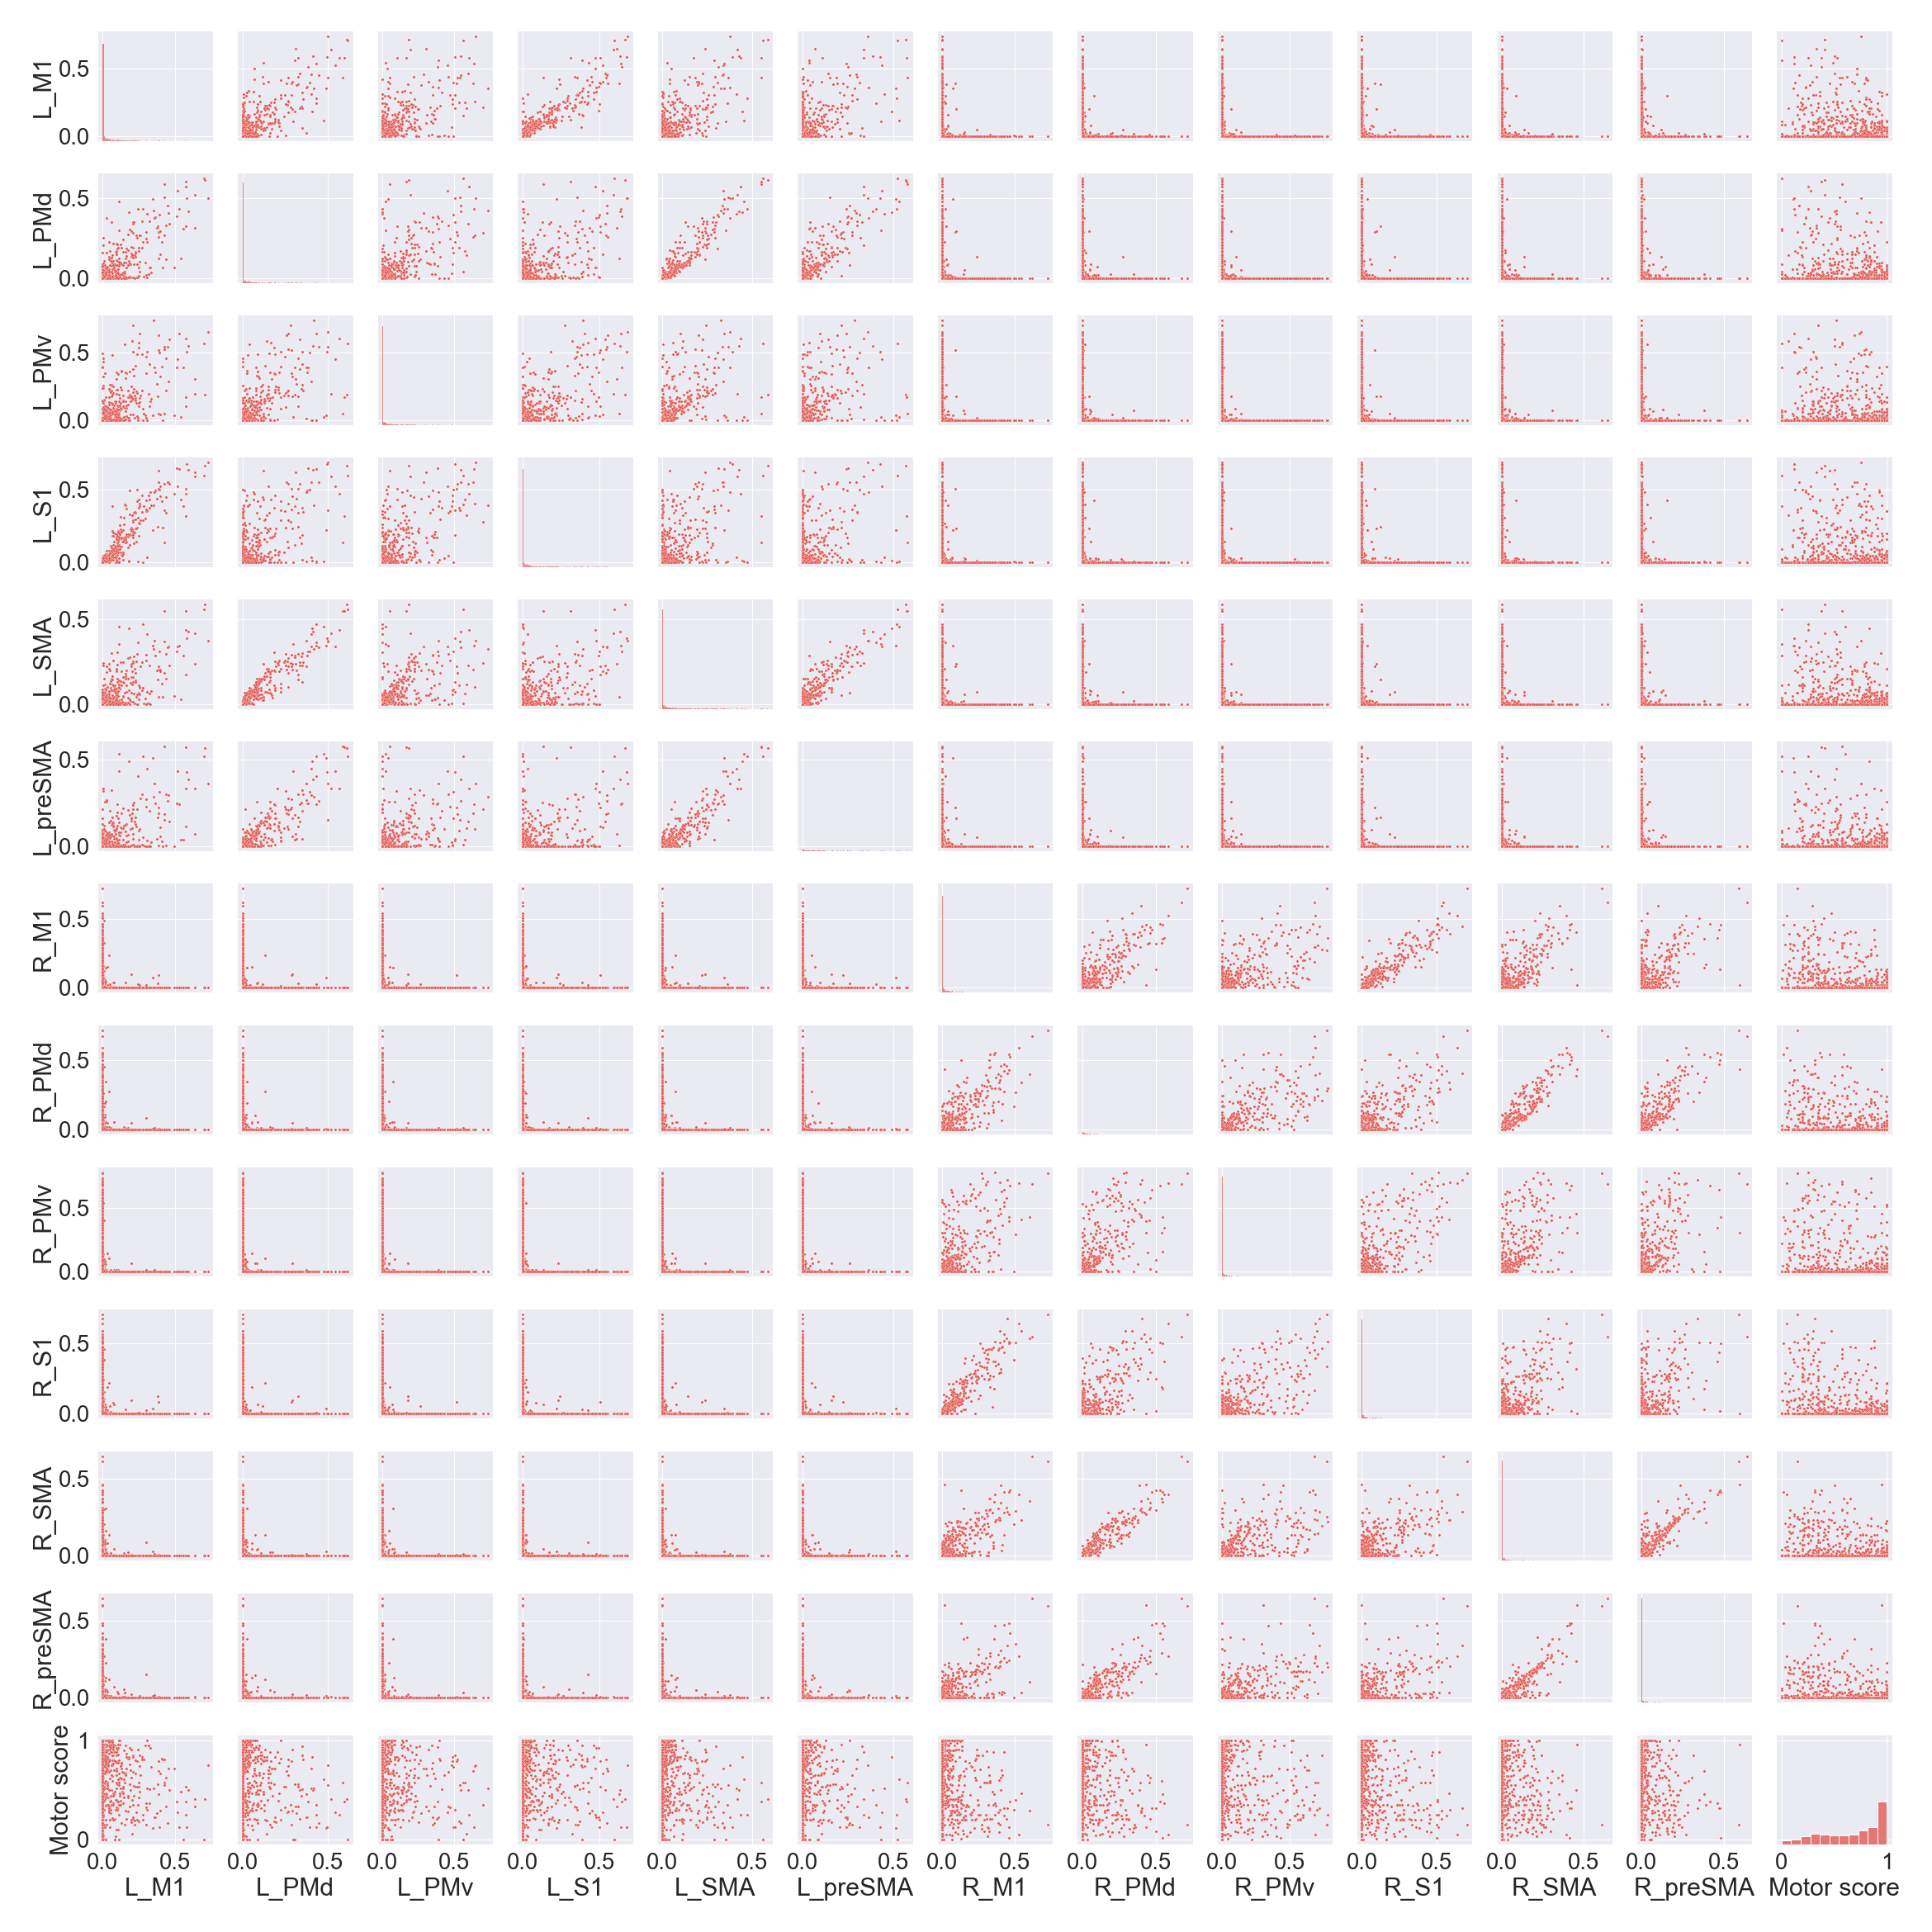
\includegraphics[width=1\linewidth]{figures/SMATT_bi_scatterplts.png}
\caption{Correlations between lesion load calculated for each left and right hemisphere tract in the sensorimotor area tract template atlas.}
\label{smatt_pairwise_correlations_bi}
\end{figure}


\begin{table}[h]
\centering
\caption{Results training on acute and chronic data, testing only on chronic data.}
\label{table:5}
\begin{tabular}{lrrrr}
\toprule
 &  & \multicolumn{2}{c}{Median performance} \\
 Ensembele type & Model name & Corr. (Std. dev.) & $R^2$ (Std. dev.) \\
\midrule
\multirow[t]{6}{*}{None} & M1 CST LL & 0.394 (0.004) & 0.142 (0.004) \\
 & Ipsi. SMATT LL & 0.430 (0.004) & 0.174 (0.004) \\
 & L/R SMATT LL & 0.446 (0.006) & 0.188 (0.006) \\
 & sLNM LL & 0.427 (0.007) & 0.165 (0.007) \\
 & ChaCo (shen268) & 0.456 (0.012) & 0.199 (0.014) \\
 & ChaCo (fs86) & 0.457 (0.008) & 0.203 (0.009) \\
 \arrayrulecolor{black!30}\midrule
\multirow[t]{6}{*}{Demographics} & M1 CST LL $\Plus$ demog. & 0.424 (0.005) & 0.173 (0.004) \\
 & Ipsi. SMATT LL $\Plus$ demog. & 0.457 (0.006) & 0.199 (0.004) \\
 & L/R SMATT LL $\Plus$ demog. & 0.462 (0.007) & 0.203 (0.004) \\
 & sLNM LL $\Plus$ demog. & 0.452 (0.006) & 0.191 (0.004) \\
 & ChaCo (shen268) $\Plus$ demog. & 0.468 (0.009) & 0.204 (0.007) \\
 & ChaCo (fs86) $\Plus$ demog. & 0.471 (0.007) & 0.203 (0.005) \\
 \arrayrulecolor{black!30}\midrule
\multirow[t]{4}{*}{chaco ll} & M1 CST LL $\Plus$ ChaCo (fs86) & 0.448 (0.005) & 0.199 (0.005) \\
 & Ipsi. SMATT LL $\Plus$ ChaCo (fs86) & 0.462 (0.006) & 0.212 (0.006) \\
 & L/R SMATT LL $\Plus$ ChaCo (fs86) & 0.469 (0.005) & 0.219 (0.005) \\
 & sLNM LL $\Plus$ ChaCo (fs86) & 0.467 (0.006) & 0.214 (0.007) \\
 \arrayrulecolor{black!30}\midrule
\multirow[t]{4}{*}{chaco ll demog} & M1 CST LL $\Plus$ ChaCo  (fs86) $\Plus$ demog. & 0.473 (0.006) & 0.212 (0.005) \\
 & Ipsi. SMATT LL $\Plus$ ChaCo  (fs86) $\Plus$ demog. & 0.489 (0.006) & 0.228 (0.005) \\
 & L/R SMATT LL $\Plus$ ChaCo  (fs86) $\Plus$ demog. & 0.491 (0.006) & 0.228 (0.005) \\
 & sLNM LL $\Plus$ ChaCo  (fs86) $\Plus$ demog. & 0.485 (0.006) & 0.221 (0.005) \\
\bottomrule
\end{tabular}
\end{table}






\end{document}